\documentclass[conference]{IEEEtran}
\IEEEoverridecommandlockouts
% The preceding line is only needed to identify funding in the first footnote. If that is unneeded, please comment it out.
\usepackage{cite}
\usepackage{amsmath,amssymb,amsfonts}
\usepackage{algorithmic}
\usepackage{graphicx}
\usepackage{textcomp}
\usepackage{xcolor}
\usepackage{url}
% Name of the framework. Change it here to rename it everywhere.
\newcommand{\fw}{AEGIS}
\def\BibTeX{{\rm B\kern-.05em{\sc i\kern-.025em b}\kern-.08em
    T\kern-.1667em\lower.7ex\hbox{E}\kern-.125emX}}
\begin{document}

\title{Does Horizon-Informed Gradient Weighting Help a Learnable Climate-Delay Encoder? A Leakage-Controlled Study of District-Level Dengue Forecasting in Sri Lanka}

\author{\IEEEauthorblockN{Kulathunge K. A. N. H.}
\IEEEauthorblockA{\textit{Dept. of Computer Science and Engineering} \\
\textit{University of Moratuwa}\\
Moratuwa, Sri Lanka \\
nadilk.23@cse.mrt.ac.lk}
\and
\IEEEauthorblockN{Angeesa R. P. T.}
\IEEEauthorblockA{\textit{Dept. of Computer Science and Engineering} \\
\textit{University of Moratuwa}\\
Moratuwa, Sri Lanka \\
thilokyaa.23@cse.mrt.ac.lk}
\and
\IEEEauthorblockN{Gunaweera N.}
\IEEEauthorblockA{\textit{Dept. of Computer Science and Engineering} \\
\textit{University of Moratuwa}\\
Moratuwa, Sri Lanka \\
nethsithg.23@cse.mrt.ac.lk}
\and
\IEEEauthorblockN{Mallawarachchi H. S.}
\IEEEauthorblockA{\textit{Dept. of Computer Science and Engineering} \\
\textit{University of Moratuwa}\\
Moratuwa, Sri Lanka \\
hesandim.23@cse.mrt.ac.lk}
\and
\IEEEauthorblockN{Wijesekara M. S. T.}
\IEEEauthorblockA{\textit{Dept. of Computer Science and Engineering} \\
\textit{University of Moratuwa}\\
Moratuwa, Sri Lanka \\
senilkam.23@cse.mrt.ac.lk}
% TODO: add the TA and supervisor author blocks here.
}

\maketitle

\begin{abstract}
Weather affects dengue with a delay of several weeks. A forecaster that learns these delays should therefore learn them from forecasts made far enough ahead for the delay to matter. In a normal multi-horizon network, however, the delay encoder is trained by the losses of all horizons, including short horizons that barely use weather. We test a training strategy for this problem. Inside the training years, we measure how much each forecast horizon relies on correctly timed weather. We then use these measurements to weight the gradients that reach only the climate encoder. All other parts of the network keep the normal, equally weighted loss. We use weekly dengue counts for 25 districts of Sri Lanka and forecast 1--4 weeks ahead. The evaluation is walk-forward, and we fixed the decision rules before scoring. The weighted model did not beat an identical model trained with equal weights. Its mean absolute error changed by +0.06 to +0.08 cases per district-week, which is within noise at every horizon. This happened even though the weights differed by up to four times between horizons. Diagnostics show why the effect was small: the weighting turns each update by only about 7\textdegree{} and changes its size by about 13\%, and the two trained models differ less than two random seeds of the same model. In exploratory tests, training the climate encoder from the 4-week loss alone gave the lowest error, while GradNorm-style balancing was worse than equal weights. We report the main result as negative and treat the routing result as a lead that still needs confirmation.
\end{abstract}

\begin{IEEEkeywords}
dengue forecasting, multi-horizon forecasting, gradient weighting, multi-task learning, climate delay, recurrent neural networks
\end{IEEEkeywords}

\section{Introduction}

Dengue control in Sri Lanka needs lead time. Vector control teams need weeks to act, and hospitals need time to plan staff and beds. The 2017 epidemic was the largest on record~\cite{weng2024graph}, and it showed the cost of acting late. A useful forecast must therefore work several weeks ahead, not only one.

Weather is the natural source of this lead time. Rain and temperature affect mosquito breeding and virus development after a delay. For Sri Lankan districts, climate lags of 7--9 weeks have been used~\cite{liu2025explainable}. But the value of weather depends on the forecast horizon. At one week ahead, the latest case count already holds almost all of the signal. In our preliminary experiments on the same case data, removing all climate inputs changed the one-week error by only 0.01 cases per district-week. At four weeks, breaking the timing of the weather removed about half of the model's gain over persistence.

This creates a training problem. A multi-horizon network usually shares one encoder across all horizons and trains it on one combined loss. If this encoder must learn weather delays, most of its training signal comes from horizons where weather timing hardly matters. Our preliminary results show the effect. A learnable delay encoder trained at one week ahead learned delays that did not match the delays measured from the data, and it was less accurate than fixed, hand-chosen windows.

Existing tools do not target this case directly. Multi-task balancing methods such as GradNorm~\cite{chen2018gradnorm} and uncertainty weighting~\cite{kendall2018multi} reweight task losses for all shared parameters, using statistics from the current training run. Gradient routing~\cite{cloud2024gradient} controls which data update which parameters, but it was proposed to localise abilities inside a network, not to improve forecasts. We did not find a study that sets horizon weights from an out-of-sample measurement and applies them to one input encoder only.

We therefore ask a narrow question: \emph{does weighting the gradients that reach only a learnable climate encoder, by how much each horizon relies on climate, improve multi-horizon dengue forecasts compared with an identical model trained with equal weights?}

To answer it, we build a two-branch network that forecasts 1--4 weeks ahead. One branch reads case history. The other branch reads weather through learnable delay kernels for each district. We measure each horizon's reliance on climate inside the training years and send the weighted loss to the climate encoder only. We then compare this model with an equal-weight twin in a walk-forward evaluation, using decision rules that we fixed before scoring any test year.

Our contributions are:
\begin{enumerate}
\item \textbf{A controlled test of a training strategy, with a negative result.} We compare out-of-sample, horizon-specific gradient weighting of one input encoder with an identical equal-weight model. The weighting gave no useful improvement, although the weights were up to four times apart.
\item \textbf{Measurements of what the weighting changes.} We measure its effect on each optimiser update and on the trained model, and compare both with the variation between random seeds.
\item \textbf{Exploratory evidence on gradient routing.} Training the climate encoder from the longest horizon alone gave the lowest error. GradNorm applied to the same encoder did not help. These results are not yet confirmed.
\end{enumerate}

\section{Related Work}

\textbf{Neural dengue forecasting.} Recent dengue forecasters combine a recurrent encoder over time with spatial structure and climate inputs. Graph neural networks have been used for the 25 districts of Sri Lanka and were reported to beat ARIMA, random forest and LSTM models~\cite{weng2024graph}. DengueGNN combines dynamic graph convolution with attention-based LSTMs across several countries~\cite{gulmohamed2026denguegnn}. A hybrid SEIR--LSTM model links climate and social factors to dengue in 16 merged regions of Sri Lanka~\cite{liu2025explainable}. These studies show that a recurrent encoder is a natural backbone, and our model uses one. They differ in how clearly they separate the effect of each part. For example, DengueGNN reports no persistence baseline, and none of its ablations removes the graph completely~\cite{gulmohamed2026denguegnn}. We therefore compare with persistence and with a matched model that differs from ours only in the training strategy.

\textbf{Delayed climate effects.} Epidemiology models delayed weather effects with distributed lag non-linear models (DLNMs)~\cite{gasparrini2010dlnm}. These estimate how risk changes with both the exposure and the lag. A DLNM study of dengue in Barbados found that delays differ by variable: about five months for drought and one to two months for heavy rain~\cite{lowe2018barbados}. Neural forecasters usually fix the lags before training. One study selects lagged climate inputs for 27 Brazilian states and explains them with SHAP~\cite{chen2025climatespatial}. Another selects 7--9-week lags for Sri Lanka~\cite{liu2025explainable}. We take two ideas from this work: delays can be long, and they differ by variable. Our encoder therefore learns a separate, smooth delay kernel for each district and variable, in a similar way to the smooth lag basis of a DLNM. Unlike these approaches, it learns the delays inside the network, which raises the question of which horizon's loss should train them.

\textbf{Multi-horizon forecasting and count likelihoods.} Direct multi-horizon models predict all horizons from one encoder, as in MQ-RNN~\cite{wen2017mqrnn} and the Temporal Fusion Transformer~\cite{lim2021tft}. DeepAR uses a recurrent network with a Negative Binomial likelihood for count data~\cite{salinas2020deepar}. Our model uses both ideas: one direct head per horizon and a Negative Binomial output. Neither is a contribution of this paper. In these models all horizons share one combined loss. We did not find work on \emph{which} horizons should train a given input encoder.

\textbf{Loss balancing and gradient routing.} When tasks share parameters, one task can dominate or conflict with another. Some methods adapt the loss weights during training. GradNorm tunes gradient sizes so that tasks train at similar rates~\cite{chen2018gradnorm}, and uncertainty weighting learns weights from task uncertainty~\cite{kendall2018multi}. Other methods change the gradients themselves: PCGrad removes the conflicting part of each task gradient~\cite{yu2020pcgrad}. Gradient routing masks gradients so that chosen data update chosen parts of the network~\cite{cloud2024gradient}. Our method sits between these groups. Like GradNorm, it weights task losses. Like gradient routing, it sends the weighted loss to one part of the network. It differs in the source of the weights: a measurement on held-out years inside the training period, not statistics from the current run. We include GradNorm as a comparison, because it is the closest established method.

\section{Methodology}

This section introduces \fw{}, a general framework for training forecasting networks that predict several steps ahead and use \emph{driver series}. We describe it in general terms, so it can be applied to any temporal data with the same structure. Section~\ref{sec:setup} shows how we apply it to dengue forecasting.

The idea behind the framework is simple. In many forecasting problems there is a \emph{main series} that we want to predict and one or more \emph{driver series} that affect it after a delay. Rainfall affects river flow a few days later, temperature affects electricity demand, and weather affects disease cases several weeks later. A driver of this kind often matters little for the next step, because the latest value of the main series already tells us most of what we need. It matters much more for forecasts further ahead. A normal multi-horizon network trains its driver encoder with the losses of all horizons added together. Most of the encoder's training signal can therefore come from horizons that hardly use the drivers. \fw{} changes this. It first measures how much each horizon relies on the drivers, and then lets each horizon train the driver encoder in proportion to that reliance. The rest of the network is trained in the usual way.

Fig.~\ref{fig:framework} gives an overview. The framework has three steps:
\begin{enumerate}
\item a \emph{two-branch forecaster} that keeps the driver series in their own encoder;
\item a \emph{measurement step} that estimates how much each horizon relies on the drivers, using training data only;
\item a \emph{training rule} that uses these measurements to weight the gradients that reach the driver encoder, and only the driver encoder.
\end{enumerate}

% ---------------------------------------------------------------------------
% FIGURE BRIEF (for generating Fig. framework later; this comment is not printed)
% ---------------------------------------------------------------------------
% Layout: one wide figure (full page width), three panels from left to right,
% connected by large arrows. Light background, flat style, rounded boxes.
% Colour code (use the same colours everywhere, including the caption):
%   BLUE   (#2E6FD8) = main series and the history branch
%   ORANGE (#F28C28) = driver series and the driver encoder
%   PURPLE (#7B4FC9) = the measurement step (Step 2)
%   RED    (#D7263D) = the weighted loss L_drv and its gradients
%   GREY   (#7A7A7A) = the ordinary equal-weight loss L_equal and its gradients
%   GREEN  (#2A9D5C) = the final forecasts
%
% Panel (a) "Step 1: Two-branch forecaster"
%   - Top-left input: a small BLUE line chart labelled "Main series y (recent W steps)".
%   - Bottom-left input: two or three small ORANGE line charts stacked, labelled
%     "Driver series x (V variables)".
%   - BLUE path: input -> box "Per-unit layers" -> box "GRU" -> label "history state".
%   - ORANGE path: input -> box "Lag kernels" with a small picture of a smooth bump
%     curve over a lag axis (0 ... L), made of 2-3 faint Gaussian bumps adding to one
%     solid curve -> box "GRU" -> label "driver state".
%     Next to the lag kernel, draw a timeline with the forecast origin t and the
%     target week t+h; shade the allowed lags (>= h before t+h) and grey out the
%     future part, with a small note "only data known at t".
%   - Both paths meet in a box "Gate g_h" (a small dial/valve icon) that scales the
%     orange correction before adding it to the blue correction.
%   - Output: an "anchor" icon labelled "start from latest value y_t", plus the two
%     corrections, giving GREEN forecast bars "h = 1, 2, ..., H".
%
% Panel (b) "Step 2: Measure reliance (training data only)"
%   - A timeline of the training period split into K coloured inner blocks
%     (train | early stop | score). Test years shown greyed out and crossed, with
%     the note "test data never used".
%   - A PURPLE box "Pilot model (equal weights)".
%   - Two scoring routes: "real drivers" (normal orange chart) and
%     "seasonal swap" (the same chart with a segment cut out and replaced by a
%     segment from another year at the same season, shown with a curved swap arrow).
%   - Result: a small PURPLE bar chart "reliance u_h" rising from h = 1 to h = H,
%     then an arrow to a second bar chart "weights w_h" (mean 1, floor epsilon shown
%     as a thin dashed line).
%
% Panel (c) "Step 3: Driver-only weighted training"
%   - The same two-branch network as in (a), drawn smaller.
%   - Per-horizon losses L_1 ... L_H as small boxes on the right.
%   - GREY arrows: all L_h with equal weight -> "L_equal" -> back into the BLUE
%     branch, the gate and the heads.
%   - RED arrows of different thickness (thin for h = 1, thick for h = H, matching
%     the weights from panel (b)) -> "L_drv" -> back into the ORANGE driver encoder only.
%   - A small "lock" icon on the BLUE branch next to the red arrows, meaning
%     "the weighted loss does not reach this part".
%   - A footnote box: "All w_h = 1 -> ordinary training (baseline)".
%
% Optional bottom strip (one line of small icons): examples of main/driver pairs
% from other fields to show generality: "cases <- weather", "electricity load <-
% temperature", "river flow <- rainfall", "sales <- promotions".
% ---------------------------------------------------------------------------
\begin{figure*}[htbp]
\centerline{\fbox{\parbox{0.95\textwidth}{\centering\vspace{2.2cm}\textit{Framework diagram to be added (see the figure brief in the source).}\vspace{2.2cm}}}}
\caption{Overview of the \fw{} framework. (a)~A two-branch forecaster: the history branch (blue) reads the recent main series, and the driver encoder (orange) reads the driver series through learnable lag kernels. A gate decides, for each horizon, how much of the driver correction to add to a forecast that starts from the latest observed value. (b)~Inside the training period only, pilot models measure how much each horizon relies on correctly timed drivers (purple); the reliance values become horizon weights. (c)~During training, the weighted loss (red) updates only the driver encoder, while the ordinary equal-weight loss (grey) updates every other part. With all weights equal to one, this is ordinary training.}
\label{fig:framework}
\end{figure*}

\subsection{Problem Setting}

We have $N$ units observed at regular time steps. A unit can be a region, a sensor, a store or a patient group. For unit $i$ at time $t$, $y_{i,t}$ is the value of the main series and $\mathbf{x}_{i,t}\in\mathbb{R}^{V}$ holds the values of $V$ driver variables. At a forecast origin $t$, the model may use only data up to time $t$. It predicts $y_{i,t+h}$ for every unit and every horizon $h \in \{1,\dots,H\}$. All horizons are predicted directly and at once from the same origin; one forecast is not fed into the next.

The framework is meant for problems with three properties: several horizons share one network, the drivers act with a delay, and the drivers matter more for some horizons than for others. Step~2 checks the third property from the data.

\subsection{Step 1: A Two-Branch Forecaster}

The forecaster has two branches (Fig.~\ref{fig:framework}a). The split keeps the parameters that learn from the drivers apart from the rest of the network, so that Step~3 can train them differently.

\textbf{History branch.} This branch reads the last $W$ steps of the main series for each unit, together with simple context inputs such as the time of year and missing-data flags. Small per-unit layers feed a recurrent encoder, a GRU~\cite{cho2014gru}. Its output summarises the recent behaviour of the main series.

\textbf{Driver encoder.} This branch reads the driver series. It first has to answer the question \emph{how far back should the model look?} For every unit $i$ and driver variable $v$, it learns a \emph{lag kernel} $k_{i,v}(\ell)$. The kernel is a set of non-negative weights over the lags $\ell = 0, \dots, L$ that sum to one. It turns the driver history into one smoothed value,
\begin{equation}
\tilde{x}_{i,v} = \sum_{\ell} k_{i,v}(\ell)\, x_{i,v,\tau-\ell}, \label{eq:kernel}
\end{equation}
where $\tau$ is the time step the lags are counted from (see below). To keep the kernel smooth, we build it as a mixture of $M$ Gaussian bumps:
\begin{equation}
k_{i,v}(\ell) = \sum_{m=1}^{M} \pi_{i,v,m}\, b_m(\ell), \qquad
\boldsymbol{\pi}_{i,v} = \mathrm{softmax}\!\left(\mathbf{e}_i^{\top} P_v\right). \label{eq:mixture}
\end{equation}
Each bump $b_m$ is a Gaussian over the lags, with a learned centre and width that all units and variables share. The vector $\mathbf{e}_i$ is a learned embedding of unit $i$, and $P_v$ is a learned projection for variable $v$. As a result, different units and different variables can learn different delays, while the number of parameters stays small. The smoothed driver values then pass through a small recurrent encoder. We call the lag kernels and this recurrent encoder together the \emph{driver encoder}, with parameters $\theta_{\mathrm{drv}}$.

\textbf{Target-relative lags.} We count lags back from the step being predicted, $\tau = t+h$, not from the origin $t$. For horizon $h$, the kernel may use only lags of at least $h$. It therefore reads only driver values that are already known at the origin, and it is renormalised over these allowed lags. One kernel serves all horizons, and each horizon uses its own allowed part of it. This has two benefits. The model never sees future data, and a learned lag means the same thing at every horizon: a lag of eight steps always means ``eight steps before the predicted step''. The framework also allows \emph{origin-relative} lags as an alternative. In that case, one kernel looks back from the origin, all horizons share it, and the number of parameters is the same.

\textbf{Combining the branches.} For each horizon, the history branch gives a correction $\delta^{\mathrm{hist}}_h$ and the driver encoder gives a correction $\delta^{\mathrm{drv}}_h$. A gate $g_h \in (0,1)$ decides how much of the driver correction to use. It is computed from the history state, a unit bias and a horizon bias. The forecast starts from the latest observed value and moves away from it:
\begin{equation}
\log \mu_h = \log(1+y_t) + \delta^{\mathrm{hist}}_h + g_h\,\delta^{\mathrm{drv}}_h . \label{eq:mean}
\end{equation}
If both corrections are zero, the forecast is simply the latest value plus one. The network therefore only has to learn how the future differs from the present. Here $\mu_h$ is the mean of the predictive distribution. For count data we use a Negative Binomial distribution, as in DeepAR~\cite{salinas2020deepar}; other kinds of data can use another distribution without changing the rest of the framework. The point forecast is the median of the distribution.

\subsection{Step 2: Measuring How Much Each Horizon Relies on the Drivers}

Step~3 needs a weight $w_h$ for each horizon that says how useful the drivers are at that horizon. The weights must not use test data, so we measure them inside the training period (Fig.~\ref{fig:framework}b):
\begin{enumerate}
\item Split the training period into $K$ inner blocks. Each block has its own training span, early-stopping period and scoring period.
\item In each block, train a \emph{pilot model} with ordinary equal weights.
\item Score each pilot twice on its scoring period. The first score uses the real drivers. For the second score, replace each unit's driver window with the same unit's window from another year, taken at the same point in the season. This \emph{seasonal swap} keeps the usual seasonal pattern but breaks the exact timing of the drivers.
\item The \emph{shuffle reliance} of horizon $h$ is the increase in error, $g_h = \mathrm{MAE}_{\mathrm{swapped}} - \mathrm{MAE}_{\mathrm{real}}$. We average it over seeds and blocks, and clip it at zero to get $u_h$.
\end{enumerate}
The weights are
\begin{equation}
w_h = \varepsilon + (1-\varepsilon) \cdot \frac{H\,u_h}{\sum_k u_k}. \label{eq:weights}
\end{equation}
A horizon that relies more on the drivers gets a larger weight. The weights have a mean of one, and every horizon keeps a weight of at least $\varepsilon$, so no horizon is cut off completely. Shuffle reliance measures how much a trained model depends on correctly timed drivers. It is not a causal effect of the drivers.

\subsection{Step 3: Driver-Only Weighted Training}

Let $L_h$ be the loss at horizon $h$ (the negative log-likelihood, computed over observed values only), and let $a_h$ be the share of all observed values that fall at horizon $h$, so that $\sum_h a_h = 1$. We define two losses:
\begin{equation}
L_{\mathrm{equal}} = \sum_h a_h L_h, \qquad
L_{\mathrm{drv}} = \frac{\sum_h a_h w_h L_h}{\sum_h a_h w_h}. \label{eq:loss}
\end{equation}
$L_{\mathrm{equal}}$ is the ordinary training loss. $L_{\mathrm{drv}}$ is the same loss with the horizon weights from Step~2. Training then works as follows (Fig.~\ref{fig:framework}c). After one forward pass, the driver encoder $\theta_{\mathrm{drv}}$ receives the gradient of $L_{\mathrm{drv}}$. All other parameters, namely the history branch, the gate and every prediction head, receive the gradient of $L_{\mathrm{equal}}$. One gradient-norm clip and one optimiser step follow.

The weighting therefore changes only \emph{what the driver encoder learns}. Each prediction head is still trained by its own unweighted loss, so no horizon is given up to help another. When all $w_h = 1$, the update is exactly the ordinary update. We checked this numerically. Any standard multi-horizon model is therefore a special case of the framework, which makes it a clean baseline.

\subsection{Choices Within the Framework}

The framework separates the \emph{measurement} of the weights (Step~2) from the \emph{training rule} that uses them (Step~3). Different choices can therefore be compared while everything else stays fixed:
\begin{itemize}
\item \textbf{How the weights are set:} equal weights (the baseline); measured weights (Eq.~\eqref{eq:weights}, the proposed rule); fixed weights chosen by hand; \emph{hard routing}, where only the longest horizon trains the driver encoder; or weights learned during training, as in GradNorm~\cite{chen2018gradnorm}.
\item \textbf{How reliance is measured:} the seasonal swap above, or another measure, such as the gain of a pilot over a pilot without drivers.
\item \textbf{How lags are aligned:} target-relative or origin-relative.
\end{itemize}

\textbf{Applying the framework to other data.} To use \fw{} in a new setting, one chooses the main series, the driver series, the horizons and a suitable output distribution. Steps~2 and~3 then run unchanged, because they need only a set of horizon losses and a way to swap driver windows. In this paper we test one instance of the framework, on dengue data; the next section describes it.

\section{Experimental Setup}\label{sec:setup}

\textbf{Applying \fw{} to dengue forecasting.} We test the framework on district-level dengue forecasting in Sri Lanka. The units are the 25 districts, the main series is the weekly number of confirmed dengue cases, and the drivers are seven weather variables. We forecast $H = 4$ horizons, 1--4 weeks ahead. Weather affects mosquito breeding and virus development after a delay of several weeks~\cite{liu2025explainable,lowe2018barbados}, so this setting has the three properties the framework needs. Because the drivers are weather, we call the driver encoder the \emph{climate encoder} and its loss $L_{\mathrm{clim}}$ in the rest of the paper.

\textbf{Data.} Weekly confirmed dengue counts come from the denguedatahub package~\cite{talagala2026denguedatahub}. We merge 26 reporting areas into the 25 districts of Sri Lanka, which gives 1,012 weeks from December 2006 to May 2026. Daily weather comes from the ERA5 reanalysis~\cite{munoz2021era5land}, taken from the Open-Meteo archive~\cite{openmeteo2026historical}. We sample it at each district's centroid and sum or average it over each reporting week. Missing targets are masked, never filled in. Missing inputs are filled from a district-by-month average over the training years and flagged.

\textbf{Model settings.} The network has 10,028 parameters.
\begin{itemize}
\item \emph{History (case) branch.} Each district's last 12 weeks enter as nine inputs: log cases, the season (sine and cosine of the day of the year), missing-data flags, the district's coordinates, its weekly rank among all districts, and its total cases over the past 52 weeks. Two per-district layers feed a GRU with 32 units. The branch has no graph layer. In our preliminary experiments, graphs based on shared borders, on distance, or learned from data never beat this per-district model.
\item \emph{Climate encoder.} The seven weather variables are rainfall, the share of rainy days, temperature, daily temperature range, dew point, relative humidity and wind speed. They enter over 37 weeks. Each district and variable has a lag kernel over delays of 0--29 weeks, built from $M = 6$ Gaussian bumps. We use softmax instead of a sparse alternative because, in preliminary tests, sparsemax and entmax left most kernels with zero gradient. The climate GRU has 16 units.
\item \emph{Output.} The sum of the two corrections in Eq.~\eqref{eq:mean} is clipped to $[-10, 10]$. $\mu_h$ is the mean of a Negative Binomial (NB2) distribution, and the case branch predicts its dispersion.
\end{itemize}

\textbf{Measuring the weights.} We use $K = 3$ inner blocks in each fold and train each pilot with two seeds. The seasonal swap takes each district's weather window from another year, within $\pm$2 weeks of the same season, and is repeated five times. We set $\varepsilon = 0.05$, so with $H = 4$ Eq.~\eqref{eq:weights} becomes $w_h = 0.05 + 0.95 \cdot 4u_h / \sum_k u_k$.

\textbf{Compared models.} The \emph{equal-weight model} (B) is the main baseline. It is identical to the \emph{utility-weighted model} (D) except for the weights, so the comparison shows the effect of the training rule alone. Table~\ref{tab:arms} lists the other arms, which cover the choices in the previous section. They answer four questions: does the lag alignment matter, do the weights need to be measured, does a harder routing rule work better, and how does an established balancing method compare?

\begin{table}[htbp]
\caption{Comparison Arms}
\begin{center}
\begin{tabular}{|c|c|p{3.9cm}|}
\hline
\textbf{Arm} & \textbf{Delays} & \textbf{What trains the climate encoder}$^{\mathrm{a}}$ \\
\hline
B & target & equal weights (baseline) \\
D & target & shuffle-reliance weights (proposed) \\
A & origin & equal weights \\
C & origin & shuffle-reliance weights \\
E & target & fixed weights 1:2:3:4 \\
F & target & only the 4-week loss \\
G & target & weights from gain over a case-only pilot \\
H & target & GradNorm~\cite{chen2018gradnorm} \\
\hline
\multicolumn{3}{l}{$^{\mathrm{a}}$In all arms, the heads and case branch use $L_{\mathrm{equal}}$.}
\end{tabular}
\label{tab:arms}
\end{center}
\end{table}

We also report two outside references, which are not controlled ablations. The first is \emph{persistence}, which repeats the latest count; at short horizons, every model must beat it. The second is Chronos-2~\cite{ansari2025chronos2}, a pretrained time-series model used zero-shot, with no training on our data. It shows how accurate our small models are compared with a large general model.

\textbf{Splits.} We use nine expanding walk-forward folds with test years 2017--2025. Training data end two years before each test year, and the year in between is used for validation. Each cell belongs to a split by its target week. Results average the seven \emph{headline} years (2017--2019 and 2022--2025). The COVID years 2020--2021 appear only in a robustness check. All methods are scored on the same 11,725 cells per horizon. The first 19 weeks of 2026 give a further hold-out check.

\textbf{Training.} We use Adam~\cite{kingma2015adam} with a batch size of 64 and at most 150 epochs. The gradient-norm clip is 1.0. The delay kernels use a learning rate of $2\times10^{-2}$ without weight decay. All other parameters use $3\times10^{-3}$ with weight decay $10^{-4}$. Early stopping (patience 15) uses the \emph{unweighted} validation likelihood, so the choice of model does not depend on the weights we test. The main comparison uses five seeds per arm. The exploratory arms use three seeds, and each is compared with B on the same three seeds. The full study needed 583 training runs and 93.9 GPU-minutes on one laptop GPU (RTX 4070 Laptop). One forecast for 25 districts and four horizons takes 2.4\,ms.

\textbf{Metrics.} The main metric is the mean absolute error (MAE) in cases per district-week. \emph{Peak MAE} is the MAE on district-weeks at or above the district's 90th percentile of past cases, so it measures accuracy in high-incidence weeks. A model's score is the mean of its scores over seeds.

\textbf{Statistics and decision rules.} We compare paired differences over the seven years with t-tests and apply a Holm correction over the four horizons~\cite{holm1979simple}. Confidence intervals (CIs) come from a bootstrap that resamples 4-week blocks of origins, with all districts kept together. Before scoring any test year, we fixed these rules. \emph{Improvement} needs D$-$B $\le -0.30$ MAE at 3 or 4 weeks, with Holm-adjusted $p<0.05$ and a 95\% CI below zero. \emph{Non-inferiority} at 1--2 weeks needs the upper CI bound to be at most $+0.30$. Any other outcome is \emph{no measurable difference}. The other arms are exploratory, and their tests are not adjusted.

\textbf{Protocol history.} We fixed the arms, seeds, folds, weights and decision rules before scoring any test year. After we had seen the first results, we found an implementation error: the climate correction head had received weighted gradients instead of unweighted ones. We fixed it and re-ran the affected arms with the same rules. The main conclusion did not change, and all results below come from the corrected runs. Because we had already seen the data, these are corrected evaluations of past data, not a blind test. This also applies to 2026.

\section{Results}

\subsection{The Baseline Is a Strong Reference}

Table~\ref{tab:accuracy} compares the equal-weight model with the outside references. B has a higher MAE than persistence at one week. From two weeks on, its MAE is lower, and at four weeks it is 3.2 cases per district-week below persistence. At 3--4 weeks, B is within 0.25 MAE of a separately trained Negative Binomial GRU. At every horizon it is within 0.7 MAE of Chronos-2. The main comparison is therefore made against a strong model.

\begin{table}[htbp]
\caption{Headline MAE (Cases per District-Week)}
\begin{center}
\begin{tabular}{|l|c|c|c|c|c|}
\hline
\textbf{Method} & \multicolumn{4}{|c|}{\textbf{Horizon (weeks)}} & \textbf{Peak} \\
\cline{2-5}
 & \textbf{\textit{1}} & \textbf{\textit{2}} & \textbf{\textit{3}} & \textbf{\textit{4}} & \textbf{\textit{4 wk}} \\
\hline
Persistence & 16.42 & 20.16 & 24.58 & 28.47 & 47.98 \\
NB GRU$^{\mathrm{a}}$ & 15.94 & 19.26 & 22.46 & 25.07 & 42.60 \\
Chronos-2$^{\mathrm{b}}$ & 15.96 & 19.07 & 22.29 & 25.11 & 43.74 \\
B (equal) & 16.64 & 19.67 & 22.71 & 25.22 & 42.99 \\
D (utility) & 16.70 & 19.75 & 22.78 & 25.28 & 42.81 \\
\hline
\multicolumn{6}{l}{$^{\mathrm{a}}$Separate model per horizon; reference, not an ablation.} \\
\multicolumn{6}{l}{$^{\mathrm{b}}$Zero-shot, joint over districts.}
\end{tabular}
\label{tab:accuracy}
\end{center}
\end{table}

\subsection{The Weights Were Far from Uniform}

Shuffle reliance was highest at four weeks in all ten folds, and it increased with every horizon step in nine of them (Fig.~\ref{fig:weights}). The weights therefore favoured the longest horizon by a factor of 1.7--4.0 over the shortest. In the 2022 fold, for example, they were 0.46, 0.81, 1.18 and 1.54 for horizons 1--4. The other utility, the gain over a pilot without weather (arm G), was small and changed sign across folds, from $-0.03$ to $+0.12$. Its weights were therefore very uneven and changed from fold to fold (Fig.~\ref{fig:weights}, right).

\begin{figure*}[htbp]
\centerline{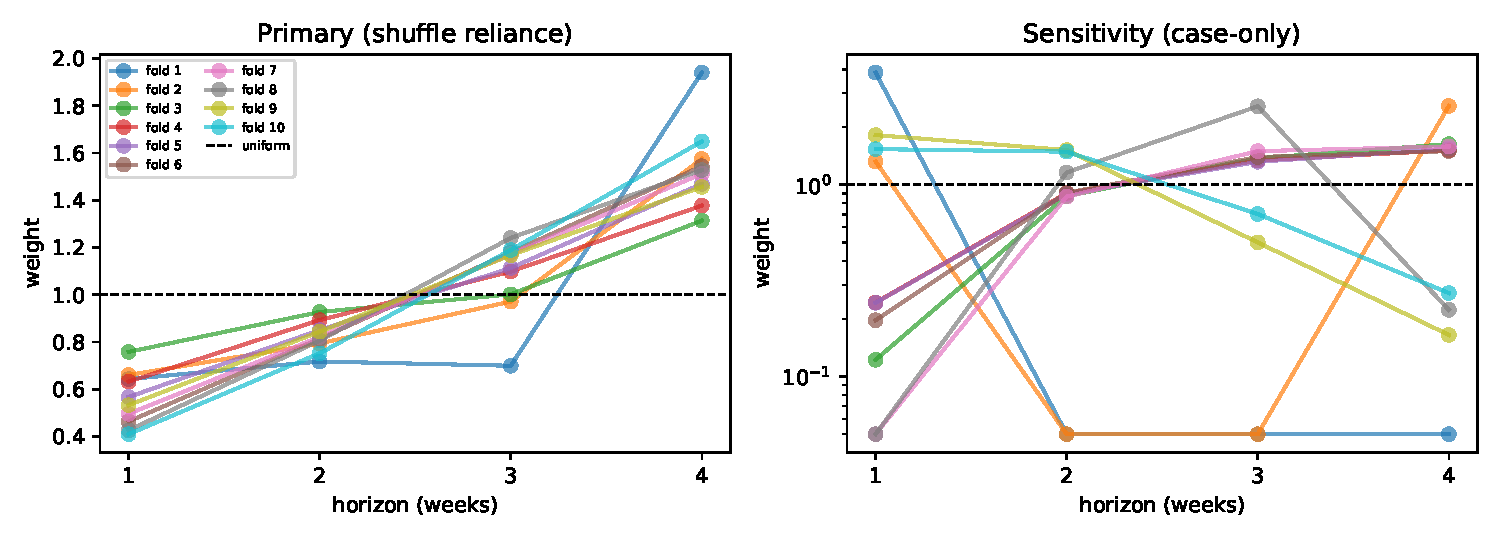
\includegraphics[width=0.85\textwidth]{figures/weights_vs_uniform.pdf}}
\caption{Frozen weights per horizon for each fold. Left: shuffle-reliance weights used by D. Right: case-only weights used by G (log scale). The dashed line marks equal weights.}
\label{fig:weights}
\end{figure*}

\subsection{Utility Weighting Did Not Improve the Forecasts}

Table~\ref{tab:primary} gives the main result. D had a slightly higher error than B at every horizon, and no difference was significant. Under the fixed rules, D is non-inferior to B at 1--2 weeks, and there is no measurable difference at 3--4 weeks. The improvement rule was not met. The result stays the same when we score the seed-averaged forecast ($+0.06$), when we include the COVID years ($+0.05$ to $+0.07$), and when we use longer bootstrap blocks. In the 2026 hold-out, D was again worse than B at every horizon ($+0.18$ to $+0.50$). This check agrees in sign, but it is not blind.

\begin{table}[htbp]
\caption{Main Comparison: D$-$B, Headline MAE, Five Seeds}
\begin{center}
\setlength{\tabcolsep}{3pt}
\begin{tabular}{|c|c|c|c|c|}
\hline
\textbf{Horizon} & \textbf{D$-$B}$^{\mathrm{a}}$ & \textbf{Holm $p$} & \textbf{95\% CI} & \textbf{Verdict} \\
\hline
1 wk & $+0.06$ & 0.72 & $[-0.03, +0.17]$ & non-inferior \\
2 wk & $+0.08$ & 0.44 & $[-0.03, +0.21]$ & non-inferior \\
3 wk & $+0.07$ & 0.72 & $[-0.07, +0.23]$ & no difference \\
4 wk & $+0.06$ & 0.72 & $[-0.10, +0.22]$ & no difference \\
\hline
\multicolumn{5}{l}{$^{\mathrm{a}}$Negative values favour D.}
\end{tabular}
\label{tab:primary}
\end{center}
\end{table}

\subsection{Exploratory Arms}

Table~\ref{tab:explore} compares each exploratory arm with B on the same three seeds. Arm F, where only the 4-week loss trains the climate encoder, had the lowest error at every horizon. It beat B by 0.64--0.69 MAE and was better in five or six of the seven years. Its CIs exclude zero at 1--2 weeks ($[-1.26, -0.20]$ at one week) but include zero at 3--4 weeks ($[-1.70, +0.41]$ at four weeks). Weights from the gain over a case-only pilot (G) and GradNorm (H) were both worse than B at every horizon. The delay alignment changed the effect of weighting. With origin-relative delays, measured weighting (C) had a lower MAE than B, while equal weighting (A) had a higher MAE. With target-relative delays, D and B were equal. In a post-hoc 2$\times$2 analysis over all nine folds, the interaction between weighting and alignment was $+0.58$ MAE at four weeks (95\% CI $[+0.26, +0.91]$). No fold-level test survived Holm correction, and most of the effect came from 2017 and 2019.

\begin{table}[htbp]
\caption{Change in Headline MAE Relative to B (Same Seeds)}
\begin{center}
\begin{tabular}{|l|c|c|c|c|}
\hline
\textbf{Arm} & \multicolumn{4}{|c|}{\textbf{Horizon (weeks)}$^{\mathrm{a}}$} \\
\cline{2-5}
 & \textbf{\textit{1}} & \textbf{\textit{2}} & \textbf{\textit{3}} & \textbf{\textit{4}} \\
\hline
A: origin, equal & $+0.24$ & $+0.27$ & $+0.44$ & $+0.50$ \\
C: origin, measured & $-0.40$ & $-0.42$ & $-0.31$ & $-0.27$ \\
E: fixed 1:2:3:4 & $-0.06$ & $-0.11$ & $-0.09$ & $-0.12$ \\
F: 4-week loss only & $\mathbf{-0.65}$ & $\mathbf{-0.69}$ & $\mathbf{-0.66}$ & $\mathbf{-0.64}$ \\
G: case-only gain & $+0.62$ & $+0.58$ & $+0.70$ & $+0.80$ \\
H: GradNorm & $+0.12$ & $+0.11$ & $+0.18$ & $+0.11$ \\
\hline
\multicolumn{5}{l}{$^{\mathrm{a}}$Negative values favour the arm. Tests are not adjusted.}
\end{tabular}
\label{tab:explore}
\end{center}
\end{table}

\subsection{How Much the Weighting Changes Training}

To see why D and B behave alike, we compared their gradients at 60 matched training states, each with the same model, optimiser state and batch (Table~\ref{tab:diag}). The weighting turned the climate-encoder update by about 7\textdegree{} on average and changed its size by 13\%. The raw gradient norm grew by 14.7\%, but the Adam update norm grew by only 2.6\%. In the trained models, B and D differ less from each other than two seeds of B do, both in their forecasts and in their learned kernels. The learned rainfall kernels centre at 8--10 weeks, and D's kernels sit about 0.7 weeks later than B's. They agree only weakly with a cross-correlation scan of each district's rainfall and cases over the training years (Spearman 0.15--0.31). The climate gate rises with the horizon, from 0.43 at one week to 0.56 at four weeks, and B and D differ by at most 0.02.

\begin{table}[htbp]
\caption{Size of the Change Caused by Utility Weighting}
\begin{center}
\begin{tabular}{|p{4.6cm}|c|}
\hline
\textbf{Quantity} & \textbf{Value} \\
\hline
Angle between D and B updates (mean) & 7.1\textdegree{} (2.8--13.9\textdegree) \\
Relative update difference $\|u_D-u_B\|/\|u_B\|$ & 13.1\% (5--24\%) \\
Forecast difference: B vs.\ D & 1.7--2.9 cases \\
Forecast difference: two seeds of B & 3.5--5.2 cases \\
Rainfall-kernel L1 distance: B vs.\ D & 0.41 \\
Rainfall-kernel L1 distance: two seeds of B & 0.72 \\
\hline
\end{tabular}
\label{tab:diag}
\end{center}
\end{table}

\section{Discussion}

\textbf{What the result means.} For this model and data, weighting the climate encoder by measured horizon reliance does not improve forecasts. Two simple explanations do not apply. First, the change was not too small on paper: the weights were up to four times apart (Fig.~\ref{fig:weights}). Second, the baseline was not weak: B beats persistence from two weeks and is close to the stronger references (Table~\ref{tab:accuracy}). The null result therefore tells us something about the strategy itself, at least at this strength.

\textbf{Why the effect was small.} The diagnostics answer this at one level. The weighting changed each update less than a new random seed changes the whole run (Table~\ref{tab:diag}). A change this small is unlikely to give an accuracy gain that seven test years can detect. Why the change was so small is a different question, and our diagnostics do not answer it. Three explanations fit the evidence, but we did not test any of them. First, the horizons' gradients for the encoder already point partly in the same direction as the 4-week gradient (cosine 0.48--0.68 in the same diagnostics), and reweighting a sum of partly aligned vectors can only turn it a little. Second, Adam's per-parameter scaling may absorb much of a change in gradient size. The gap between the 14.7\% change in gradient and the 2.6\% change in update fits this idea, but we did not test it, for example by training with plain SGD. Third, the gate and the heads, which use the unweighted loss, may adapt to whatever the encoder produces.

\textbf{Routing versus weighting.} Arm F removes the short-horizon gradients from the climate encoder instead of reducing them. It gave the lowest error. This suggests that \emph{which} losses reach the encoder may matter more than \emph{how much} each is weighted, which is close to the idea of gradient routing~\cite{cloud2024gradient}. The evidence is weak, however. F used three seeds and unadjusted tests, its CIs at 3--4 weeks include zero, and we first saw its corrected form after the fix. One result was unexpected: F improved one-week forecasts as much as four-week forecasts, although one-week forecasts barely use weather. One possible reason is that an encoder trained on the long horizon learns a smoother weather summary, which the separately trained one-week head can still use. Another is that removing three loss terms simply regularises the encoder. We tested neither.

\textbf{Delay alignment.} Measured weighting helped only with origin-relative delays. With these delays, all horizons read the same lag positions and compete for the same kernel parameters, so balancing their losses could matter. With target-relative delays, each horizon uses its own part of the kernel, which may leave little conflict to resolve. This is a hypothesis. The interaction does not survive correction and depends mostly on two years. Origin-relative delays were also worse under equal weights, so part of the gain from weighting may only make up for that loss.

\textbf{Relation to previous work.} Loss-balancing methods set weights from statistics of the current run~\cite{chen2018gradnorm,kendall2018multi}. Our weights came from held-out reliance instead, and neither approach helped this encoder: GradNorm (H) was slightly worse than equal weights. This is one comparison on one small model, and it says nothing about these methods in the settings they were designed for. The learned kernels centre at 8--10 weeks, close to the 7--9-week lags used for Sri Lanka in~\cite{liu2025explainable}. However, they agree only weakly with our district-level scan, so we treat them as \emph{learned delay kernels}, not as a recovered biological delay. We report only the rainfall kernel, so the variable-specific delays found in~\cite{lowe2018barbados} remain untested here. Finally, B loses to persistence at one week and wins from two weeks. Like our preliminary results, this supports including persistence in dengue forecast evaluation, which~\cite{gulmohamed2026denguegnn} does not do.

\section{Limitations}

\textbf{Low power.} Seven headline years, with shared training histories, cannot separate differences much smaller than 0.3 MAE. The main null result means ``no effect of useful size'', not ``no effect''.

\textbf{Seed sensitivity.} With only the first three seeds, the sign of D$-$B reverses (about $-0.04$). All exploratory arms rely on three seeds.

\textbf{Not a blind test.} We fixed the protocol before scoring, but we fixed the implementation error after seeing results, and all data up to May 2026 had been seen. Arm F in particular needs a pre-declared test on new data, such as weeks reported after May 2026 or data from another country.

\textbf{Untested assumptions.} We assume that shuffle reliance shows where encoder gradients are useful. The weight formula and learning rates were fixed, not tuned, and a stronger weighting rule might behave differently.

\textbf{Data.} The weather is reanalysis at district centroids, downloaded in 2026. It is not what a forecaster would have had at each origin. We do not model reporting delays, and the study covers one country.

\section{Conclusion}

We tested whether weighting a learnable climate encoder's gradients by how much each horizon relies on weather improves multi-horizon dengue forecasts. Under decision rules fixed before scoring, it did not. The weighted model matched an identical equal-weight model at every horizon, even with weights up to four times apart. Our diagnostics show why the change was weak: it moves each update less than a new random seed moves the whole run. The exploratory arms gave two leads. Training the climate encoder from the longest horizon alone gave the lowest error, and measured weighting helped only with origin-relative delays. Both need confirmation on data that has not been seen. For anyone who trains small multi-horizon models, the practical lesson is simple: measure how much a training change moves the updates, and compare it with seed-to-seed variation, before you expect it to change accuracy.

% TODO: add acknowledgment if required.

\bibliographystyle{IEEEtran}
\bibliography{references}

\end{document}
